\documentclass[10pt]{article}
\usepackage[margin=17mm]{geometry}
\usepackage{graphicx,booktabs,hyperref}
\usepackage[strings]{underscore}
\setlength{\parindent}{0pt}\setlength{\parskip}{5pt}
\begin{document}
\section*{Strict subgroup support and the projected alternative}

Additional native finite audit, 2026-10-25. All seven original x-only fixtures
on both fixed n=22 reference/twist models, exact polynomial $z^{22}+z+1$,
recorded prime r, cofactor h and generator. Source input SHA prefix
95ee147e1221. Source/binary frozen before output; fresh native rerun is
byte-identical. One thread, 2-GiB address-space and 300-second caps,
shared AMD EPYC 9V74 Linux x86-64 host, correctness diagnostic only.

\begin{center}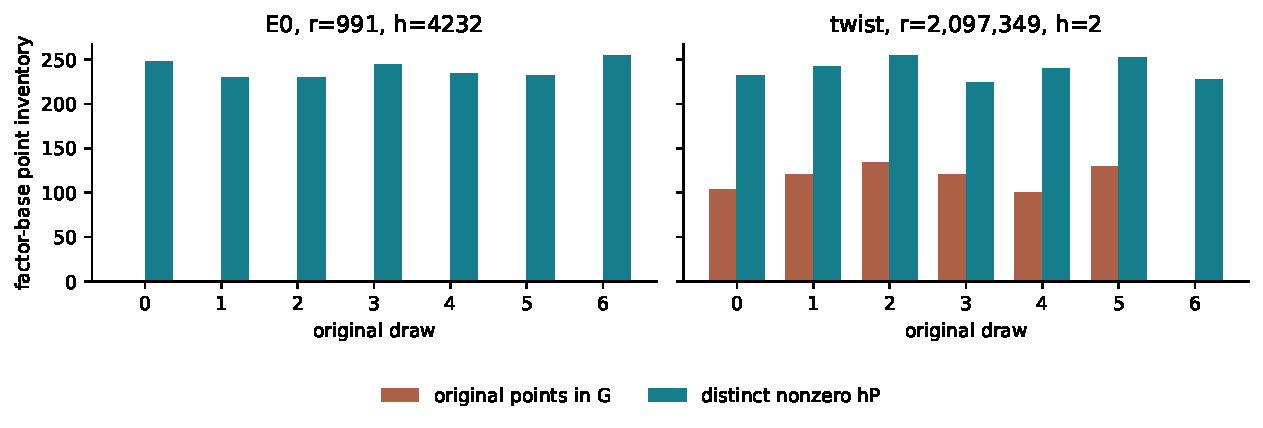
\includegraphics[width=\linewidth]{cofactor-inventories.pdf}\end{center}
The strict audit is correct about original points in G; it does not rule
out projected IC relations. Enumerating all full-curve points above V,
keeping projection multiplicities/zero images and hashing the exact distinct
inventory, gives nonempty projected bases on both models for every draw.
All projected points pass [r](hP)=O. The projected abscissae need not lie in V;
an implementation would retain the original preimage coordinates for its
algebraic oracle and the corresponding hP for logarithm variables.

For the three original SAT draws, one selected Boolean witness and one
canonical (least-y) target sign produce three verified curve relations.
All three remain verified nonzero prime-subgroup relations after multiplying
each point and target by h, although zero have every original summand in G.
The earlier audit counted both target signs; that convention gives two
relations per witness and is not contradicted by this one-sign audit.
Thus ``no original all-in-G witness'' is not a universal obstruction to IC.

Every liftable chosen-model target has nonzero hR. The E0 projected
targets for draws 0 and 1 are already in the projected base; lookup would
require its logs to have been computed and charged. Draw 6 has 254 distinct
nonzero E0 projected points despite zero original E0 points in G, and its
projected target is nonzero and not a direct projected-base hit. These are
finite support checks, not supplied discrete logarithms or measured solves.

\textbf{Open method obligations.} A projected-IC version still needs a
declared target/preimage/cofactor-component law, projected-base log collection,
exact preimage-to-projected inventory handling, scalar recovery and independent
verification, with all setup and target-dependent work charged. The original
fixtures still do not specify that complete law. This audit changes no old
strict-G receipt or Boolean count and establishes no complete-price gain,
query-rate comparison, scaling law or crossover. The 1,591/161 counts in the
separate qualified panel retain their explicitly strict-G contract.

\begin{flushleft}\footnotesize
Protocol: COFACTOR_PROJECTION_PROTOCOL.md.\par
Native receipt: \path{../../pipeline-receipts/cofactor-projection-20261025/receipt.json}\par
Exact global model identities are provided by curve-identity-adapter.v1.json.
No extra paid VM allocation or artifact upload is claimed.
\end{flushleft}

\end{document}
